% !TEX root = ../notes_unsupervisedlearning.tex
% Chapter 12: Interactive and Imitation Learning
%%%%%%%%%%%%%%%%%%%%%%%%%%%%%%%%%%%%%%%%%%%%%%%%%%%%%%%%%%%%%%%%%%%%%%

\chapter{Interactive and Imitation Learning}\index{Active Learning}\index{Imitation Learning}\index{Behavior Cloning}
\newthought{Humans correct, query, and demonstrate.}

%═══════════════════════════════════════════════════════════════════════
% BLOCK 1: INTRODUCTION
%═══════════════════════════════════════════════════════════════════════

\section{The Why}

\marginnote{Humans are expensive but informative; use them wisely.}

Sometimes the model needs guidance that cannot come from data alone. Active learning\index{active learning} queries labels for the most informative examples. Human-in-the-loop training provides continuous human correction. Imitation learning\index{imitation learning} learns from human demonstrations.

\newthought{The goal} is to maximise learning per unit of human effort.

\newthought{In order to move from passive data consumption to efficient human-guided learning} we have good reason to find ways to,
\begin{itemize}
    \item select the most informative examples for labelling so that each annotation maximises model improvement.
    \item learn policies from expert demonstrations without requiring an explicit reward function.
    \item address the covariate shift that causes imitated policies to compound small errors over time.
\end{itemize}

\subsection{Hands On Experience}

\begin{marginfigure}
\begin{tikzpicture}[scale=0.7]
    \begin{axis}[
        xlabel={$x_1$}, ylabel={$x_2$},
        xmin=0, xmax=10, ymin=0, ymax=10,
        width=\textwidth, height=\textwidth,
        axis line style={draw=none},
        tick style={black, thin},
        tick align=outside, tick pos=left,
        xtick={2,4,6,8}, ytick={2,4,6,8},
        xticklabel style={font=\tiny},
        yticklabel style={font=\tiny},
    ]
    % Decision boundary
    \addplot[black, thick, domain=0:10] {5};
    % Labeled points
    \addplot[only marks, mark=*, mark size=2pt, black] coordinates {(2,2) (3,1)};
    \addplot[only marks, mark=*, mark size=2pt, black!55] coordinates {(8,8) (7,9)};
    % Unlabeled near boundary
    \addplot[only marks, mark=o, mark size=2pt, black, thick] coordinates {
        (4,5.2) (5,4.8) (6,5.1)
    };
    % Unlabeled far from boundary
    \addplot[only marks, mark=o, mark size=1.5pt, black!30] coordinates {
        (1,1) (9,9) (2,8) (8,2)
    };
    \end{axis}
\end{tikzpicture}
\caption{Active learning: query points near the decision boundary, where uncertainty is highest.}
\label{fig:active_learning_intro}
\end{marginfigure}

You have a budget to label 5 examples. Given the current decision boundary, which points would be most valuable to label?

Points near the boundary are uncertain; labelling them helps refine the boundary. Points far from the boundary are already well-classified.

\newthought{The Learning Objectives} of this lecture:
\begin{itemize}
    \item Implement active learning with uncertainty, disagreement, and diversity sampling, and choose the appropriate strategy for a given budget.
    \item Apply behaviour cloning and DAgger for learning from demonstrations, and explain why naive cloning suffers from compounding errors.
    \item Describe inverse reinforcement learning and RLHF as methods that recover or align reward functions from human behaviour.
\end{itemize}

%═══════════════════════════════════════════════════════════════════════
% BLOCK 2: MAIN THEORY
%═══════════════════════════════════════════════════════════════════════

\newpage
\section{Active Learning}\index{active learning}

\marginnote{Choose which examples to label for maximum information gain~\cite{Settles2012ActiveLearning}.}

\subsection{Setting}

\newthought{The active learning setup:} a pool $\mathcal{U}$ of unlabelled examples, a budget $B$ for labelling queries, and the goal of maximising model performance with $B$ labels.

\subsection{Query Strategies}

\newthought{Uncertainty sampling}\index{uncertainty sampling} queries examples where the model is most uncertain:

\begin{equation}
    x^* = \arg\max_{x \in \mathcal{U}} U(f(x))
\end{equation}

Uncertainty measures include entropy $H(p) = -\sum_k p_k \log p_k$, margin $1 - (p_1 - p_2)$ where $p_1 > p_2$ are the top probabilities, and least confidence $1 - \max_k p_k$.

\newthought{Query-by-committee}\index{query-by-committee} trains an ensemble and queries where members disagree:
\begin{equation}
    x^* = \arg\max_{x \in \mathcal{U}} \text{Disagreement}(\{f_1(x), \ldots, f_M(x)\})
\end{equation}

\newthought{Diversity sampling}\index{diversity sampling} ensures queried points cover the input space:
\begin{equation}
    x^* = \arg\max_{x \in \mathcal{U}} \min_{x' \in \mathcal{L}} d(x, x')
\end{equation}

\begin{figure}
\centering
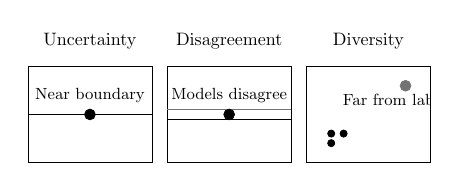
\begin{tikzpicture}[scale=0.65]
    % Uncertainty
    \begin{axis}[
        name=unc,
        title={Uncertainty},
        xmin=0, xmax=10, ymin=0, ymax=10,
        width=0.33\textwidth, ticks=none,
    ]
    \addplot[black, thick, domain=0:10] {5};
    \addplot[only marks, mark=*, mark size=3pt, black] coordinates {(5,5)};
    \node at (axis cs:5,7) {\small Near boundary};
    \end{axis}

    % Disagreement
    \begin{axis}[
        at={(unc.east)}, anchor=west, xshift=0.3cm,
        name=dis,
        title={Disagreement},
        xmin=0, xmax=10, ymin=0, ymax=10,
        width=0.33\textwidth, ticks=none,
    ]
    \addplot[black, thick, domain=0:10] {4.5};
    \addplot[black!55, thick, domain=0:10] {5.5};
    \addplot[only marks, mark=*, mark size=3pt, black] coordinates {(5,5)};
    \node at (axis cs:5,7) {\small Models disagree};
    \end{axis}

    % Diversity
    \begin{axis}[
        at={(dis.east)}, anchor=west, xshift=0.3cm,
        title={Diversity},
        xmin=0, xmax=10, ymin=0, ymax=10,
        width=0.33\textwidth, ticks=none,
    ]
    \addplot[only marks, mark=*, mark size=2pt, black] coordinates {
        (2,2) (3,3) (2,3)
    };
    \addplot[only marks, mark=*, mark size=3pt, black!55] coordinates {(8,8)};
    \node at (axis cs:8,6.5) {\small Far from labelled};
    \end{axis}
\end{tikzpicture}
\caption{Three query strategies select different points.}
\label{fig:query_strategies}
\end{figure}

\subsection{Batch Active Learning}\index{batch active learning}

\newthought{Querying multiple points at once} avoids redundancy:
\begin{equation}
    S^* = \arg\max_{S \subset \mathcal{U}, |S|=B} \text{BatchUtility}(S)
\end{equation}

Approaches include greedy selection with a diversity constraint, core-set selection, and BatchBALD.


\section{Human-in-the-Loop Learning}

\marginnote{Humans provide continuous feedback during training.}

\newthought{Feedback types} range from direct labels and corrections to comparisons where the human indicates ``A is better than B'', rankings where the human orders examples by quality, and demonstrations where the human shows how to perform a task.

\newthought{When to query:} low confidence predictions, high disagreement among models, out-of-distribution inputs, and periodic sampling for monitoring.


\section{Behavior Cloning}\index{behavior cloning}

\marginnote{Supervised learning on state-action pairs from demonstrations~\cite{Pomerleau1991ALVINN}.}

\newthought{An expert provides demonstrations} $\mathcal{D} = \{(s_1, a_1), (s_2, a_2), \ldots\}$, and the policy $\pi_\theta$ is trained to predict actions:
\begin{equation}
    \theta^* = \arg\min_\theta \sum_{(s,a) \in \mathcal{D}} \mathcal{L}(\pi_\theta(s), a)
\end{equation}

\subsection{The Covariate Shift Problem}\index{covariate shift}

\begin{figure}
\centering
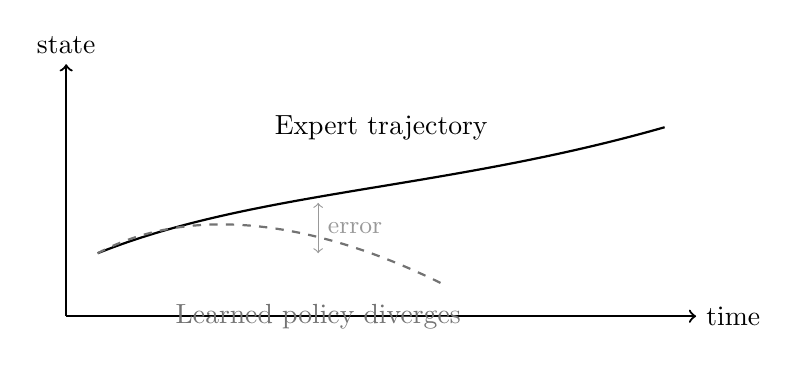
\begin{tikzpicture}[scale=0.8]
    \draw[->, thick] (0,0) -- (10,0) node[right] {time};
    \draw[->, thick] (0,0) -- (0,4) node[above] {state};

    % Expert trajectory
    \draw[black, thick] (0.5,1) .. controls (3,2) and (6,2) .. (9.5,3);
    \node at (5,3) {Expert trajectory};

    % Learned policy diverges
    \draw[black!55, thick, dashed] (0.5,1) .. controls (2,1.8) and (4,1.5) .. (6,0.5);
    \node[black!55] at (4,0) {Learned policy diverges};

    % Error compounds
    \draw[<->, black!40] (4,1.8) -- (4,1) node[midway, right] {\small error};
\end{tikzpicture}
\caption{Behaviour cloning: small errors compound, causing divergence from the expert trajectory.}
\label{fig:covariate_shift}
\end{figure}

\newthought{The problem:} the policy makes small errors that lead to states not seen in training. Performance degrades further. Errors compound exponentially.


\section{DAgger: Dataset Aggregation}\index{DAgger}

\marginnote{\newthought{DAgger.} Query the expert on the learner's state distribution~\cite{Ross2011DAgger}.}

\begin{algorithm}[H]
\caption{DAgger}
\begin{algorithmic}[1]
\State Initialize $\mathcal{D}$ with expert demonstrations
\State Train $\pi_1$ on $\mathcal{D}$
\For{$i = 1$ to $N$}
    \State Run $\pi_i$ to collect trajectories
    \State Query expert for actions at visited states
    \State Aggregate: $\mathcal{D} \gets \mathcal{D} \cup \mathcal{D}_i$
    \State Train $\pi_{i+1}$ on $\mathcal{D}$
\EndFor
\end{algorithmic}
\end{algorithm}

\newthought{The key insight:} train on states the learner actually visits, not just expert states.


\section{Inverse Reinforcement Learning}\index{inverse reinforcement learning}

\marginnote{Learn the reward function that explains expert behaviour~\cite{Ziebart2008MaxEntIRL}.}

\subsection{Motivation}

\newthought{Behaviour cloning copies actions} but does not capture why the expert acts that way. The reward function is more transferable than the policy, because it generalises to new situations.

\subsection{Maximum Entropy IRL}

\newthought{Find reward $r$} that makes the expert trajectory most likely:
\begin{equation}
    p(\tau | r) \propto \exp\left(\sum_t r(s_t, a_t)\right)
\end{equation}

Optimise:
\begin{equation}
    r^* = \arg\max_r \sum_{\tau \in \mathcal{D}_{\text{expert}}} \log p(\tau | r)
\end{equation}

\subsection{GAIL: Generative Adversarial Imitation Learning}\index{GAIL}

\marginnote{\newthought{GAIL.} Imitation as adversarial learning~\cite{Ho2016GAIL}.}

\newthought{GAIL} operates like a GAN but for trajectories: a discriminator distinguishes expert from learner trajectories, the policy tries to fool the discriminator, and no explicit reward learning is needed.


\section{Reinforcement from Human Feedback}\index{RLHF}

\marginnote{\newthought{RLHF.} How large language models learn from human preferences~\cite{Ouyang2022InstructGPT}.}

\begin{enumerate}
    \item Supervised fine-tuning: train on high-quality demonstrations
    \item Reward modelling: train a reward model on human comparisons
    \item RL fine-tuning: optimise the policy with PPO against the reward model
\end{enumerate}

\begin{figure}
\centering
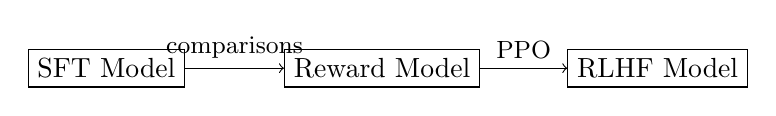
\begin{tikzpicture}[node distance=2cm]
    \node[draw, rectangle] (sft) {SFT Model};
    \node[draw, rectangle, right of=sft, xshift=1.5cm] (rm) {Reward Model};
    \node[draw, rectangle, right of=rm, xshift=1.5cm] (rlhf) {RLHF Model};

    \draw[->] (sft) -- node[above] {\small comparisons} (rm);
    \draw[->] (rm) -- node[above] {\small PPO} (rlhf);
\end{tikzpicture}
\caption{RLHF pipeline: SFT $\to$ Reward Model $\to$ RL Fine-tuning.}
\label{fig:rlhf_pipeline}
\end{figure}


%═════════════════════════════════════════════════════════���═════════════
% BLOCK 3: STUDENT ACTIVATION
%═════════════════════════════════════════��═════════════════════════════

\newpage
\section{Examples \& Exercises}

\subsection{Exercise 1: Active Learning Query}

Model outputs for 4 unlabelled points:
\begin{itemize}
    \item A: $p = [0.9, 0.1]$
    \item B: $p = [0.5, 0.5]$
    \item C: $p = [0.7, 0.3]$
    \item D: $p = [0.99, 0.01]$
\end{itemize}

Rank by uncertainty using entropy. Which would you query first?

\subsection{Exercise 2: Covariate Shift}

A self-driving car trained via behaviour cloning veers slightly right. Why does this get worse over time?

\subsection{Exercise 3: IRL vs.\ Behaviour Cloning}

When would you prefer IRL over behaviour cloning?


\section{Self-Reflection and Recap}

\newthought{Self-Reflection.}

\begin{enumerate}
    \item When does active learning provide the most benefit?
    \item Why does behaviour cloning suffer from compounding errors?
    \item How does DAgger address covariate shift, and what is its main practical limitation?
    \item When is learning a reward function more valuable than directly imitating actions?
    \item How does GAIL avoid the need for explicit reward engineering?
    \item What risks does RLHF introduce when the reward model is imperfect?
    \item How might you combine active learning with imitation learning?
\end{enumerate}

\vspace{1.5em}

\newthought{Recap.}

\begin{itemize}
    \item Active learning maximises information per label by querying uncertain, disagreed-upon, or diverse examples from the unlabelled pool.
    \item Behaviour cloning is supervised learning on demonstrations; covariate shift causes compounding errors because the learner visits states absent from expert data.
    \item DAgger mitigates covariate shift by querying the expert on states the learner actually visits, aggregating data across iterations.
    \item Inverse reinforcement learning recovers the reward function that explains expert behaviour, producing policies that transfer to new situations.
    \item RLHF aligns language models with human preferences through a learned reward model and PPO optimisation.
\end{itemize}

\vspace{2.5em}

\marginnote{\newthought{Teaser.} Interactive learning relies on human feedback. What if feedback comes as sparse rewards rather than dense supervision?}

\newthought{We have learned from human demonstrations and corrections.} But demonstrations are expensive, and in many settings the only feedback is a scalar reward after a long sequence of actions: win or lose, task success or failure, profit or loss.

\newthought{The next chapter introduces reinforcement learning,} where an agent learns to act through trial, error, and reward, without demonstrations or labelled data.

\marginnote{\newthought{feedback}}
